\documentclass{llncs}
\usepackage{array}
\usepackage{tabu}
\usepackage{amssymb}
\usepackage{graphicx}
\usepackage{color}
\usepackage{graphicx}
\usepackage{amsmath}
\usepackage{breqn}
\usepackage{epsfig}
\usepackage{cases}
\usepackage{multirow}
\usepackage{url}
\newtheorem{Definition}{Definition}
\newtheorem{Lemma}{Lemma}
\newtheorem{Theorem}{Theorem}
\newtheorem{Corollary}{Corollary}
\newtheorem{Proposition}{Proposition}
\newcommand{\shiftl}{<\hspace{-1.5mm}<}    % "squeezed" shift sign <<
\newcommand{\shiftr}{>\hspace{-1.5mm}>}    % "squeezed" shift sign <<
\newcommand{\rotl}{<\hspace{-1.5mm}<\hspace{-1.5mm}<}
\newcommand{\rotr}{>\hspace{-1.5mm}>\hspace{-1.5mm}>}
%\usepackage[left=2.7cm, right=2.7cm, top=2.7cm, bottom=2.5cm]{geometry}
\usepackage[colorlinks, bookmarks=false,pdfstartview={XYZ null null 1.50}]{hyperref}
    \hypersetup{pdffitwindow=true,linkcolor = blue,citecolor= blue,urlcolor= blue,menucolor=black} %  customize colors here
    \RequirePackage[hyperpageref]{backref}
       \renewcommand*{\backref}[1]{}
\usepackage[all]{hypcap}    %for going to the top of an image when a figure reference is clicked
\usepackage{breakurl}
\setlength{\intextsep}{10pt}
\newcommand{\ethword}{{\sf EthWord}{}}
\def\code#1{\texttt{#1}}
\begin{document}
\sloppy
\title{EthWord: A Micropayments Smart Contract}
\author{}
\institute{}
\maketitle{}
\setcounter{page}{1}
\pagenumbering{arabic}
\pagestyle{plain}
\begin{abstract}
Every blockchain transaction is verified and stored on the network nodes which maintain this decentralized system. For that, such systems sooner than later are expected to face storage scalability issues which may ultimately turn them into data center-based centralized ones. Additionally, the adoption of blockchain payments for everyday purchases is not widely convenient yet. Mainly, because a transaction requires a substantial amount of time to get confirmed on the blockchain so that a merchant is confident to get credited for the consumed goods. Accordingly, there is a strong direction to come up with cryptocurrency payment mechanisms that enable offchain irrefutable transactions which can be aggregated to fewer onchain committed ones. In this work, we propose an Ethereum-based smart contract named \ethword{} which mediates the process of conducting offchain and completely offline micropayments between two distrustful parties. More precisely, using PayWord hash chains, two parties engage in an \ethword{} smart contract which locks the exhaustion of a given chain to only one of those parties, thus enabling only such party to verify micropayments offline, and finally successfully commit aggregated transactions onchain. While other proposals allow more than two parties to get credited from one account, a continuous online monitoring of the blockchain is required in order to catch dishonest parties. However, in \ethword, no blockchain monitoring is required as a contract credits only one account.    
\\  
\textbf{Keywords:}
\end{abstract}
\section{Introduction}
\section{Background}
\ethword{} is based on the Payword micropayment technique \cite{} which relies on hash chains. A hash chain is constructed by iteratively applying a public one-way hash function $h(.)$ on a random seed value $s$. To create a hash chain of length $N$, one first selects the seed value $s$, then repeatedly applies $h(.)$ on $s$ for $N$ times, thus resulting in a sequence of $N$ hashes:
\[
h^N(s), h^{N-1}(s), h^{N-2}(s), \cdots, h^2(s), h(s),s  
\]
where $h^N(s)$ is called the tip of the chain and can be considered as the public key in a public key cryptosystem, and $s$ is also referred to by $h^0(s)$. More precisely, because of the preimage resistance of one way hash functions, knowing $h^N(s)$ does not reveal the value of $s$ or any of the previous hashes $h^{N-i}(s)$, $i=1,2,\cdots,N-1$. On the other hand, by knowing $s$ or any intermediate hash, one can easily verify the correctness of any successive hash values.

\noindent In Payword micropayment scheme, a hash chain is used as follows; the tip $h^N(s)$ is first committed by a customer by digitally signing it such that a merchant can verify this signature. Then, for each successive payment, the customer release a previous hash from the chain which can be verified by the merchant that it hashes to $h^N(s)$. Accordingly, a merchant can aggregate such individual $i$ payments and cash one equivalent larger payment by releasing $h^{N-i}(s)$ to the merchant's financial authority which can verify if it hashes iteratively for $i$ times to $h^N(s)$. The customer may use up to $N$ equivalent payments until the seed value $s$ is used. At this time the hash chain is said to be exhausted and the whole process should be re-initialized again with a different seed value. 
\section{\ethword{} Smart Contract}
\ethword{} is an Ethereum-based smart contract that enables the aggregation of an offchain set of small payments to one or more onchain larger transactions. Particularly, our contract implements a smart contract moderated version of the Payword micropayment protocol and mediates the interaction between a customer $C$ and a merchant $M$. A pseudocode for the proposed smart contract is shown in Figure \ref{fig.contract}. 
\begin{figure}[!th]
	\centering
	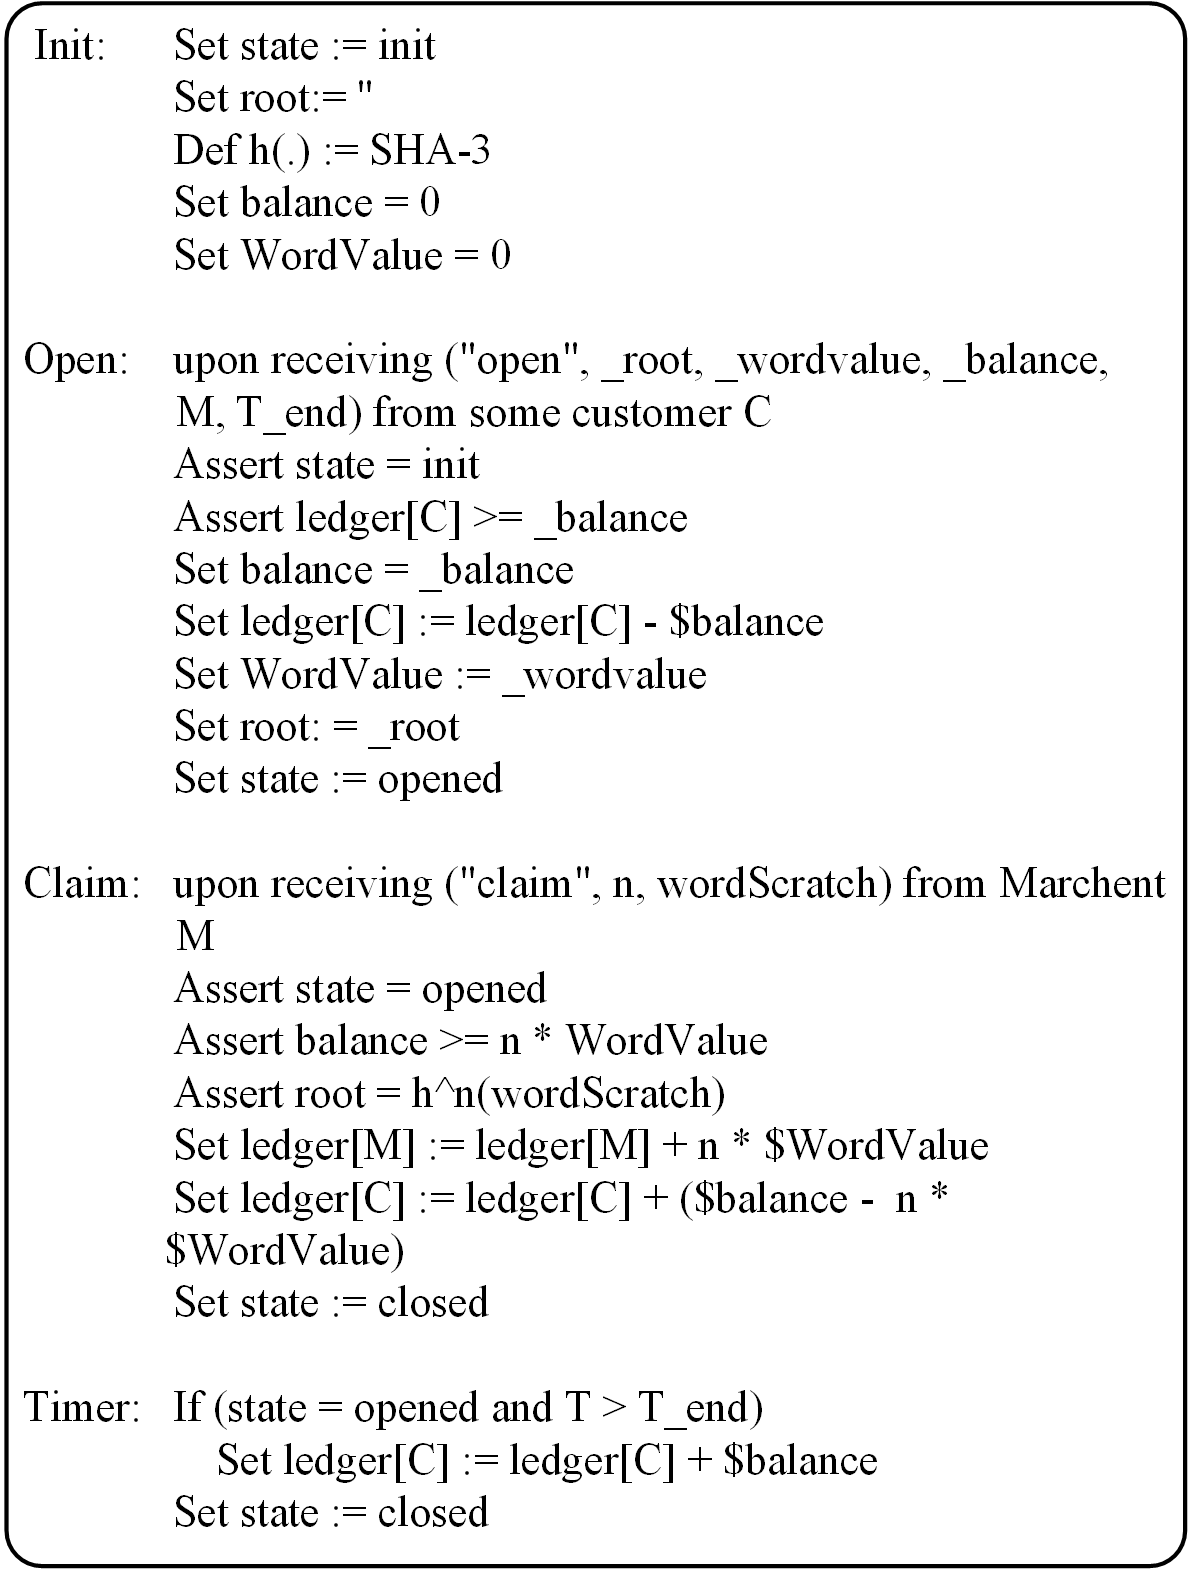
\includegraphics[scale=0.7]{pics/contract.png}
	\caption{A pseudocode for the proposed \ethword{} smart contract.}
	\label{fig.contract}
\end{figure} 

\noindent EthWord is designed with two main functions that mediate the transaction process between $C$ and $M$. First, the contract is instantiated by $C$ through calling the \code{open} function. In this function, $C$ initializes the contract through passing the pseudonym of the merchant's account $M$, the tip of the hash chain $\_root$ so that the contract can verify released intermediate hash values against it, the amount that each released hash value is worth $\_wordvalue$, and the total amount of the whole hash chain $\_balance$, and $T_{end}$ which is the time after which remaining funds in the contact's balance are refunded to the customer's account. After calling the \code{open} function, both the contract and merchant can evaluate the length of the chain and, thus, $M$ can offline know how many intermediate hash values she can accept from $C$ without the need to constantly monitor the state of the contract. Also, $M$ knows that she has to claim aggregated payments before $T_{end}$ or else, $M$ can refund the contract's available balance.
\\
\par\noindent{\textbf{Claiming aggregated payments:}} For each payment in the form of an intermediate hash $x=h^i(s)$, $i=1,2,\cdots,N-1$ that $M$ receives from $C$, she can verify its validity offline by evaluating if $h^{(N-i)}(x) = h^N(s)$ or not. Accordingly, $M$ can decide whether to accept the transaction or decline it in the event of a failed verification. After a few micropayments, where $M$ has acquired a set of intermediate hashes, she invokes the \code{claim} function in the smart contract by passing to it the last received hash value $wordScratch$, and its order within the hash chain $n$. Consequently, the contract verifies the validity and the required balance of the supplied inputs against the stored hash chain parameters, and upon successful verification, the account of $M$ is credited by the resulting balance.
\section{Security Properties}
EthWord smart contract provides the following guaranteed security properties:
\begin{itemize}
	\item Fair exchange of services:
	\item Conducting irrefutable transactions without blockchain monitoring:
\end{itemize}
%\bibliographystyle{acm}
%\bibliography{mybib}

\end{document}
